\documentclass{beamer}
\usepackage[utf8]{inputenc}
  
\usetheme{Madrid}
\usecolortheme{default}
\usepackage{amsmath,amssymb,amsfonts,amsthm}
\usepackage{txfonts}
\usepackage{tkz-euclide}
\usepackage{listings}
\usepackage{adjustbox}
\usepackage{array}
\usepackage{tabularx}
\usepackage{gvv}
\usepackage{lmodern}
\usepackage{circuitikz}
\usepackage{tikz}
\usepackage{graphicx}
\usepackage[T1]{fontenc}
\UseRawInputEncoding

\setbeamertemplate{page number in head/foot}[totalframenumber]

\usepackage{tcolorbox}
\tcbuselibrary{minted,breakable,xparse,skins}



\definecolor{bg}{gray}{0.95}
\DeclareTCBListing{mintedbox}{O{}m!O{}}{%
  breakable=true,
  listing engine=minted,
  listing only,
  minted language=#2,
  minted style=default,
  minted options={%
    linenos,
    gobble=0,
    breaklines=true,
    breakafter=,,
    fontsize=\small,
    numbersep=8pt,
    #1},
  boxsep=0pt,
  left skip=0pt,
  right skip=0pt,
  left=25pt,
  right=0pt,
  top=3pt,
  bottom=3pt,
  arc=5pt,
  leftrule=0pt,
  rightrule=0pt,
  bottomrule=2pt,
  toprule=2pt,
  colback=bg,
  colframe=orange!70,
  enhanced,
  overlay={%
    \begin{tcbclipinterior}
    \fill[orange!20!white] (frame.south west) rectangle ([xshift=20pt]frame.north west);
    \end{tcbclipinterior}},
  #3,
}
\lstset{
    language=C,
    basicstyle=\ttfamily\small,
    keywordstyle=\color{blue},
    stringstyle=\color{orange},
    commentstyle=\color{green!60!black},
    numbers=left,
    numberstyle=\tiny\color{gray},
    breaklines=true,
    showstringspaces=false,
}



\title 
{MatGeo Assignment 5.3.1}

\author
{AI25BTECH11007}
\begin{document}

\frame{\titlepage}
\begin{frame}{Question}
    For what value of k, the system of linear equations
x + y + z = 2\\
2x + y - z = 3\\
3x + 2y + kz = 4
has a unique solution?
\end{frame}

\begin{frame}{Solution}
    \[
\text{System: }
\begin{cases}
x+y+z = 2 \\
2x+y-z = 3 \\
3x+2y+kz = 4
\end{cases}
\]
\[
\mathbf A = \myvec{1\\1\\1},
 \mathbf B = \myvec{2\\1\\-1} ,
\mathbf C = \myvec{3\\2\\k},
\mathbf D = \myvec{2\\3\\4}
 \]       

\[
\text{Augmented matrix(M) : }
\myvec{A & B & C & D} = 
\myvec{1 & 1 & 1 & 2 \\ 2 & 1 & -1 & 3 \\ 3 & 2 & k & 4}
\]
\text{by row reducing,}
\[
R_2 \to R_2 - 2R_1,\quad R_3 \to R_3 - 3R_1, \quad R_3 \to R_3 - R_2
\]
\end{frame}

\begin{frame}
\[
\myvec{1 & 1 & 1 & 2 \\ 0 & -1 & -3 & -1 \\ 0 & 0 & k & -1}
\]


\begin{itemize}
\item \textbf{If \(k\neq0\):} the augmented matrix has three non-zero rows\\, so \(\operatorname{rank}(M)=3\).\\ 
hence, Unique Solution for system
\item \textbf{If \(k=0\):} the row-echelon form becomes
\[
\left[\myvec{1 & 1 & 1\\[4pt] 0 & -1 & -3\\[4pt] 0 & 0 & 0}\;\middle|\;\myvec{2\\[4pt]-1\\[4pt]-1}\right].
\]
Here \(\operatorname{rank}(M)=2\)\\
so, system is Inconsistent; No Solution.
\end{itemize}

\[
\boxed{\text{Therefore, the system has a unique solution precisely when }k\neq0.}
\]
\end{frame}

\begin{frame}{Plot}
    \begin{figure}
        \centering
        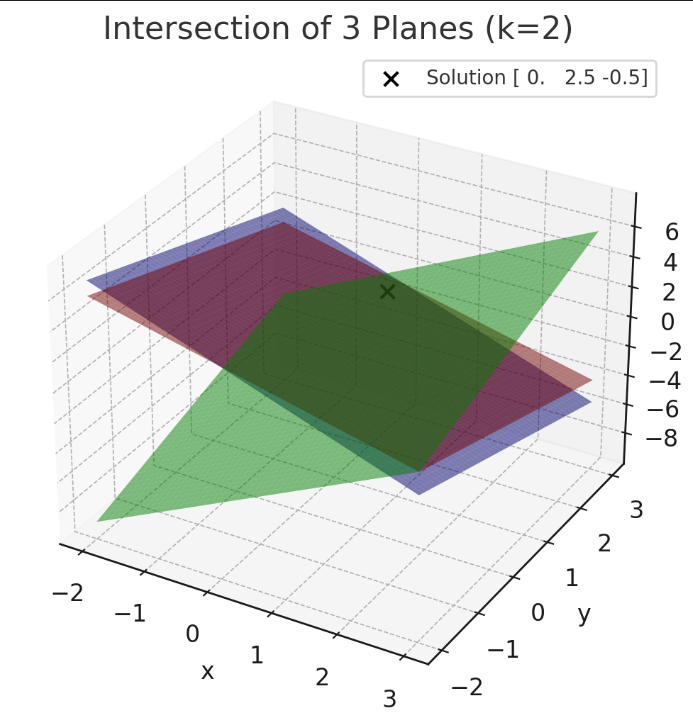
\includegraphics[width=0.75\linewidth]{figs/image.png}
        \caption{Image}
        \label{fig:placeholder}
\end{figure}
\end{frame}

\begin{frame}[fragile]{C code}
\begin{lstlisting}
    #include <stdio.h>

int main() {
    double A[3][4]; // augmented matrix [3x4]
    double k;

    // Input value of k
    printf("Enter the value of k: ");
    scanf("%lf", &k);

    // Initialize augmented matrix
    A[0][0] = 1; A[0][1] = 1;  A[0][2] = 1;  A[0][3] = 2;
    A[1][0] = 2; A[1][1] = 1;  A[1][2] = -1; A[1][3] = 3;
    A[2][0] = 3; A[2][1] = 2;  A[2][2] = k;  A[2][3] = 4;

    // Row reduction: R2 = R2 - 2*R1
    for(int j=0; j<4; j++)
        A[1][j] -= 2*A[0][j];
\end{lstlisting}
\end{frame}

\begin{frame}[fragile]{C code}
\begin{lstlisting}
    // Row reduction: R3 = R3 - 3*R1
    for(int j=0; j<4; j++)
        A[2][j] -= 3*A[0][j];
    // Row reduction: R3 = R3 - R2
    for(int j=0; j<4; j++)
        A[2][j] -= A[1][j];
    // Check k for uniqueness
    if (A[2][2] != 0) {
        printf("The system has a unique solution.\n");
        double z = A[2][3] / A[2][2];
        double y = (A[1][3] - A[1][2]*z) / A[1][1];
        double x = A[0][3] - A[0][1]*y - A[0][2]*z;

        printf("Solution: x = %.2lf, y = %.2lf, z = %.2lf\n", x, y, z);
    } else {
        printf("The system has no solution (inconsistent).\n");
    }
    return 0; }
\end{lstlisting}
\end{frame}

\begin{frame}[fragile]{Python code}
\begin{lstlisting}
    import numpy as np
import matplotlib.pyplot as plt
from mpl_toolkits.mplot3d import Axes3D

# Define k (nonzero)
k = 2

# Planes equations: coefficients and RHS
planes = [
    (np.array([1, 1, 1]), 2),    # x + y + z = 2
    (np.array([2, 1, -1]), 3),   # 2x + y - z = 3
    (np.array([3, 2, k]), 4)     # 3x + 2y + k z = 4
]

# Solve for intersection point
A = np.array([p[0] for p in planes])
b = np.array([p[1] for p in planes])
solution = np.linalg.solve(A, b)

ax.set_title(f"Intersection of 3 Planes (k={k})")

plt.show()

\end{lstlisting}
\end{frame}

\begin{frame}[fragile]{Python code}
\begin{lstlisting}
    # Create grid for plotting planes
xx, yy = np.meshgrid(np.linspace(-2, 3, 50), np.linspace(-2, 3, 50))

# Calculate corresponding z for each plane
zz1 = (2 - xx - yy)
zz2 = (3 - 2*xx - yy) * -1
zz3 = (4 - 3*xx - 2*yy) / k

# Plot planes and intersection point
fig = plt.figure(figsize=(8, 6))
ax = fig.add_subplot(111, projection='3d')

ax.plot_surface(xx, yy, zz1, alpha=0.5, color='red')
ax.plot_surface(xx, yy, zz2, alpha=0.5, color='green')
ax.plot_surface(xx, yy, zz3, alpha=0.5, color='blue')
\end{lstlisting}
\end{frame}

\begin{frame}[fragile]{python code}
    \begin{lstlisting}
        # Plot solution point
ax.scatter(*solution, color='black', s=50, label=f"Solution {solution.round(2)}")

ax.set_xlabel('x')
ax.set_ylabel('y')
ax.set_zlabel('z')
ax.legend()ame}
    \end{lstlisting}
\end{frame}


\end{document}